\chapter{Review of Heavy Flavor Results}

In the previous section, we have introduced relativistic heavy-ion physics and heavy flavor physics in vacuum and QGP. Physicists propose many experimental observables to study open heavy flavor physics and test theoretical models in heavy-ion collisions. Traditionally, heavy flavor hadron observables, such as $v_2$, $R_{AA}$, and production yield ratio, have been extensively studied. In this section, we will review selected experimental results and their comparisons with theoretical models and discuss the physics messages from the measurements.


\section{Elliptic Flow}


In the QGP medium, heavy quarks are diffused by the color force and multiple scatter with medium constituents, which could generate sizable azimuthal anisotropy $v_2$ \cite{HQReview}. In addition, due to the azimuthal anisotropic geometry of the medium, heavy quarks will have different path lengths in different directions, which will also contribute to building up $v_2$. Experimentally, we scale the $v_2$ and the hadron kinetic energy $KE_T = \sqrt{m^2 + p_T^2} - m$ of heavy quarks by $1/n_q$ according to the Number of Constituent Quark (NCQ) Scaling in quark coalescence model \cite{NCQScaling}. Figure \ref{HQV2} shows the comparison of the $v_2/n_q$ as a function of $K_T/n_q$ of $D^0$ ($c\bar u$) meson with light flavor hadrons with STAR experiments at RHIC \cite{STARD0v2} and the CMS experiment at LHC \cite{CMSD0v2}.


\begin{figure}[hbtp]
\begin{center}
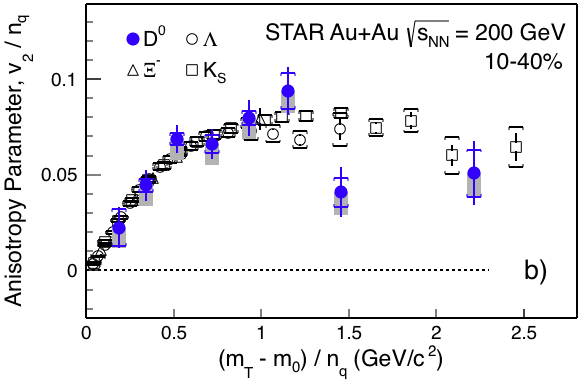
\includegraphics[width=0.50\textwidth]{Figures/Chapter2/STARv2.png}
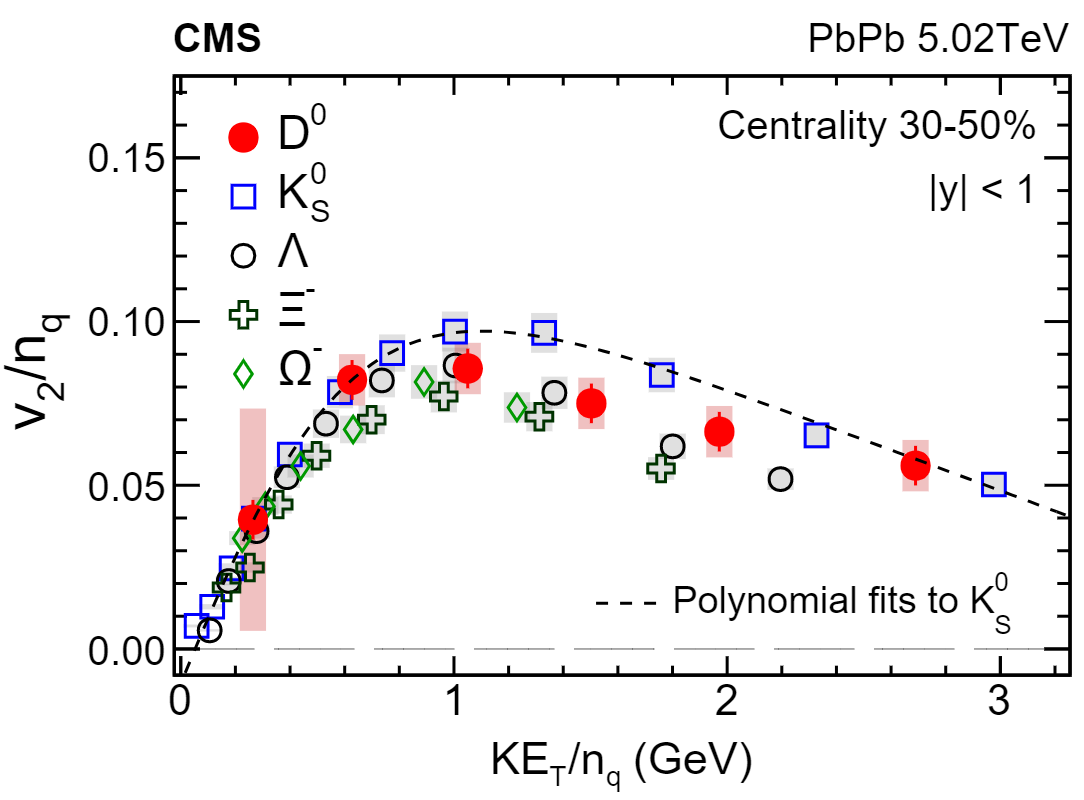
\includegraphics[width=0.485\textwidth]{Figures/Chapter2/CMSv2.png}
\caption{The NCQ scaled $D^0$ $v2/n_q$ vs $K_T/n_q$ and the comparison of light hardons measured by the STAR experiment at RHIC (left) and the CMS experiment at LHC (right) are shown above.}
\label{HQV2}
\end{center}
\end{figure}   

We could see a reasonably good NCQ scaling behavior of $D^0$ meson with other light flavor hadrons, which suggests sizable collectivity of charm quarks in the QGP medium. 

To study beauty quarks $v_2$, an indirect approach is employed. Figure \ref{BeautyEV2} shows the elliptic flow of electrons from beauty hadrons $b (\rightarrow c) \rightarrow e$ measured by the ALICE experiment \cite{ALICENPElec} and muons from beauty hadrons $b \rightarrow \mu$ measured by the ATLAS experiment \cite{ATLASNPMuon}:


\begin{figure}[hbtp]
\begin{center}
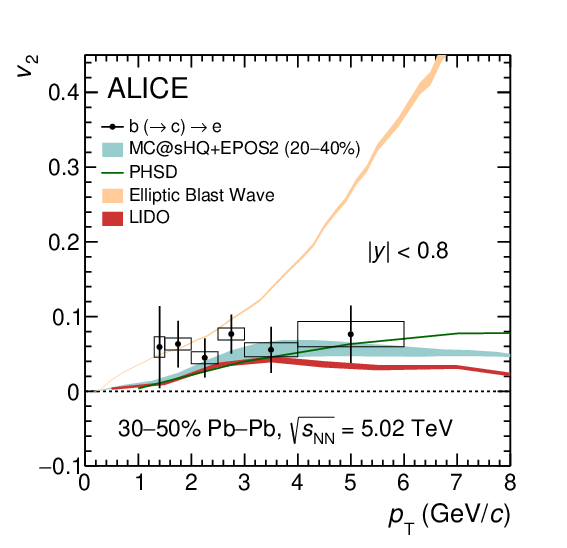
\includegraphics[width=0.44\textwidth]{Figures/Chapter2/ALICENPEv2.png}
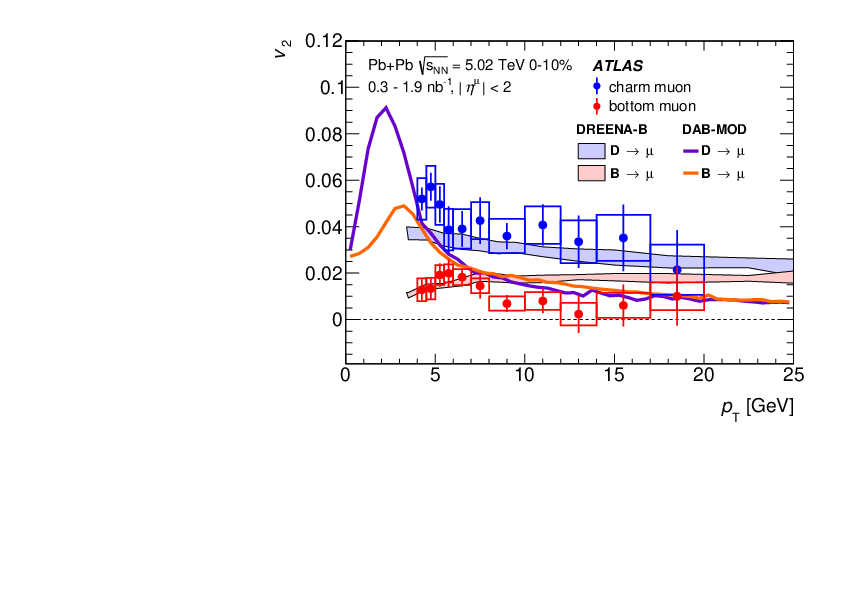
\includegraphics[width=0.52\textwidth]{Figures/Chapter2/ATLASNPMUv2.png}
\caption{The $v_2$ of electrons from b-hadron decays as a function of electron $p_T$ measured by the ALICE experiment (left) and the $v_2$ of muons from b-hadron decays as a function of muon $v_2$ measured by the ATLAS experiment (right) are shown above.}
\label{BeautyEV2}
\end{center}
\end{figure}   


Comparing Figure \ref{BeautyEV2} with Figure \ref{HQV2}, we can see that beauty quarks do not demonstrate as much anisotropy as charm quarks in heavy-ion collisions. However, so far, fully reconstructed B-meson $v_2$ has not been measured by any experiment. 



\section{Nuclear Modification Factor}

As mentioned previously, the nuclear modification factor $R_{AA}$ can describe the modification of hadron spectra in $AA$ collisions with respect to the $pp$ collisions. To study the medium modification to heavy quarks, we first would like to investigate the cold nuclear matter effect in pA collisions. Figure \ref{DRPA} and Figure \ref{BRPA} show the prompt D mesons and B mesons nuclear modification factors $R_{pA}$ in pPb collisions measured by the ALICE experiment \cite{ALICEDRPARef} and the CMS experiment \cite{CMSBRPARef} respectfully



\begin{figure}[hbtp]
\begin{center}
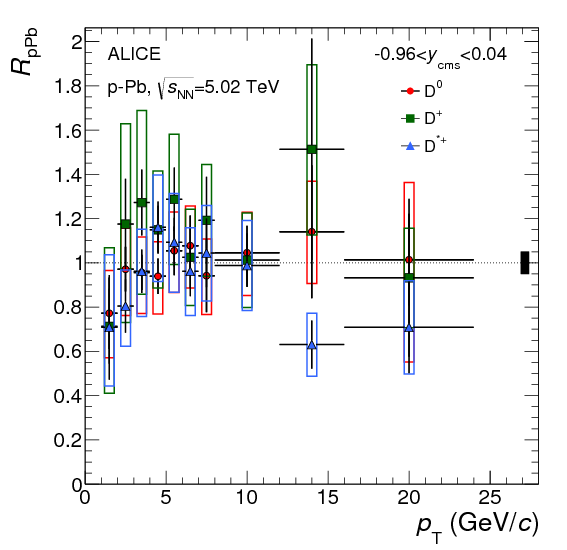
\includegraphics[width=0.60\textwidth]{Figures/Chapter2/ALICEDRpA.png}
\caption{The $R_{pA}$ as a function of $p_T$ of prompt D mesons measured by the ALICE experiment is shown above.}
\label{DRPA}
\end{center}
\end{figure}   

\begin{figure}[hbtp]
\begin{center}
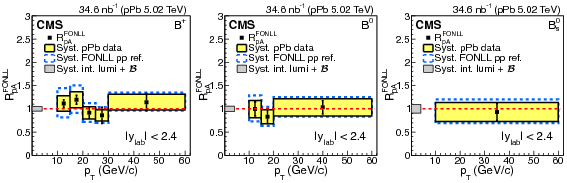
\includegraphics[width=1.10\textwidth]{Figures/Chapter2/CMSDRpA.png}
\caption{The $R_{pA}$ as a function of $p_T$ of $B^+$, $B^0$, and $B^0_s$ mesons measured by the CMS experiment is shown above.}
\label{BRPA}
\end{center}
\end{figure}   

There is no significant modification of the charm quarks due to cold nuclear matter effects since the $R_{pA}$ of $D^0$ are overall unity within experimental uncertainties. Hence, any modification of D and B mesons observed in the $AA$ collisions should come from the final state QGP effect instead of the initial state effects due to the nPDF of Pb ions. 

Next, we investigate B mesons $R_{AA}$ in the $AA$ collisions. Figure \ref{HQRAA} shows $R_{AA}$ heavy flavor hadrons measured with experiments at RHIC and LHC.

\begin{figure}[hbtp]
\begin{center}
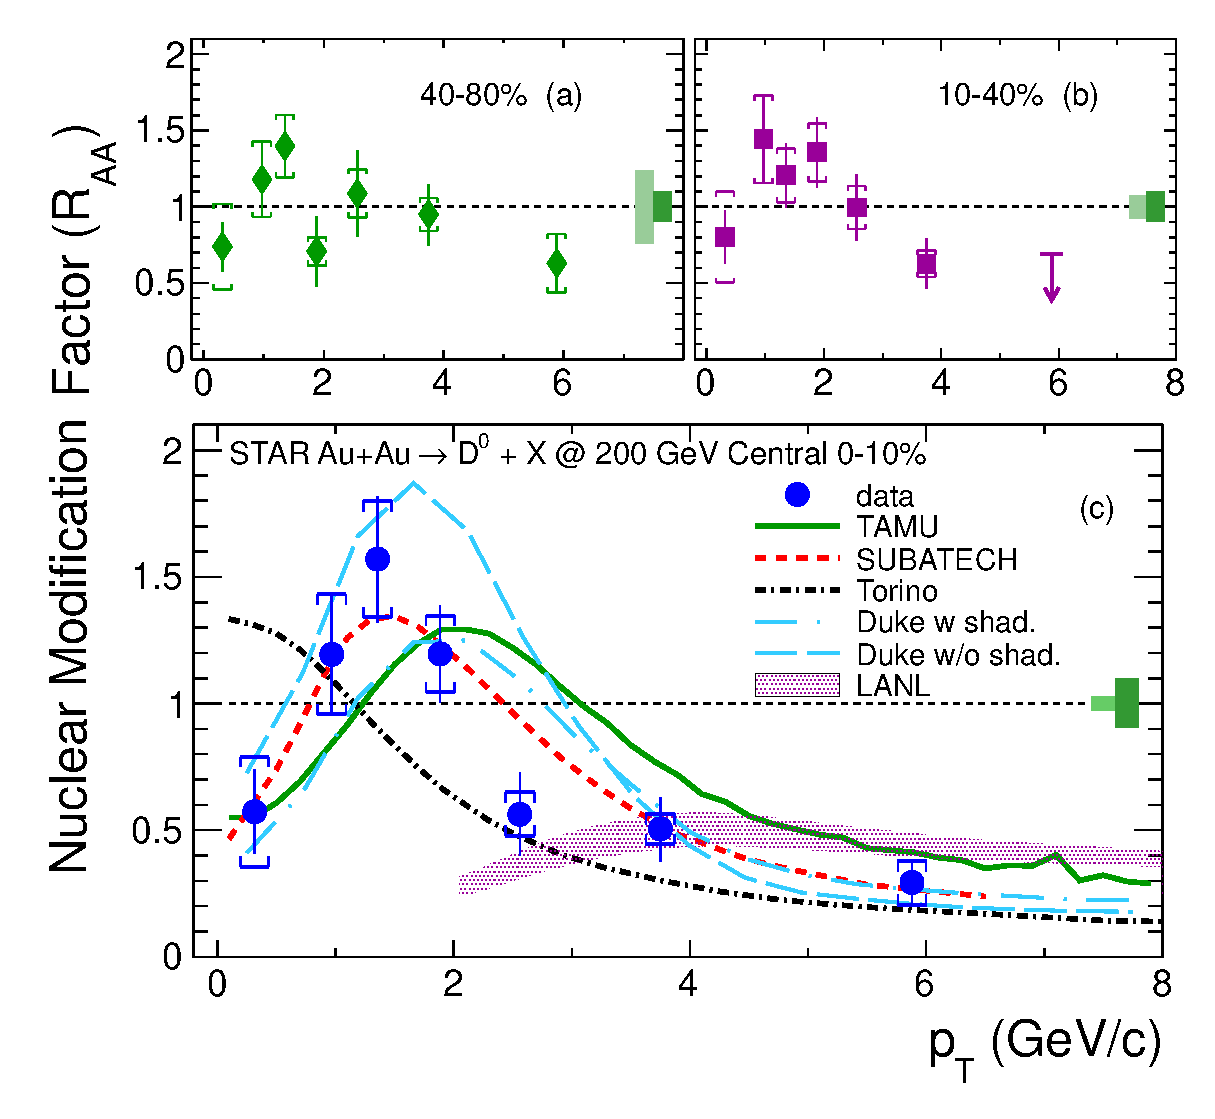
\includegraphics[width=0.47\textwidth]{Figures/Chapter2/STARRAA.eps}
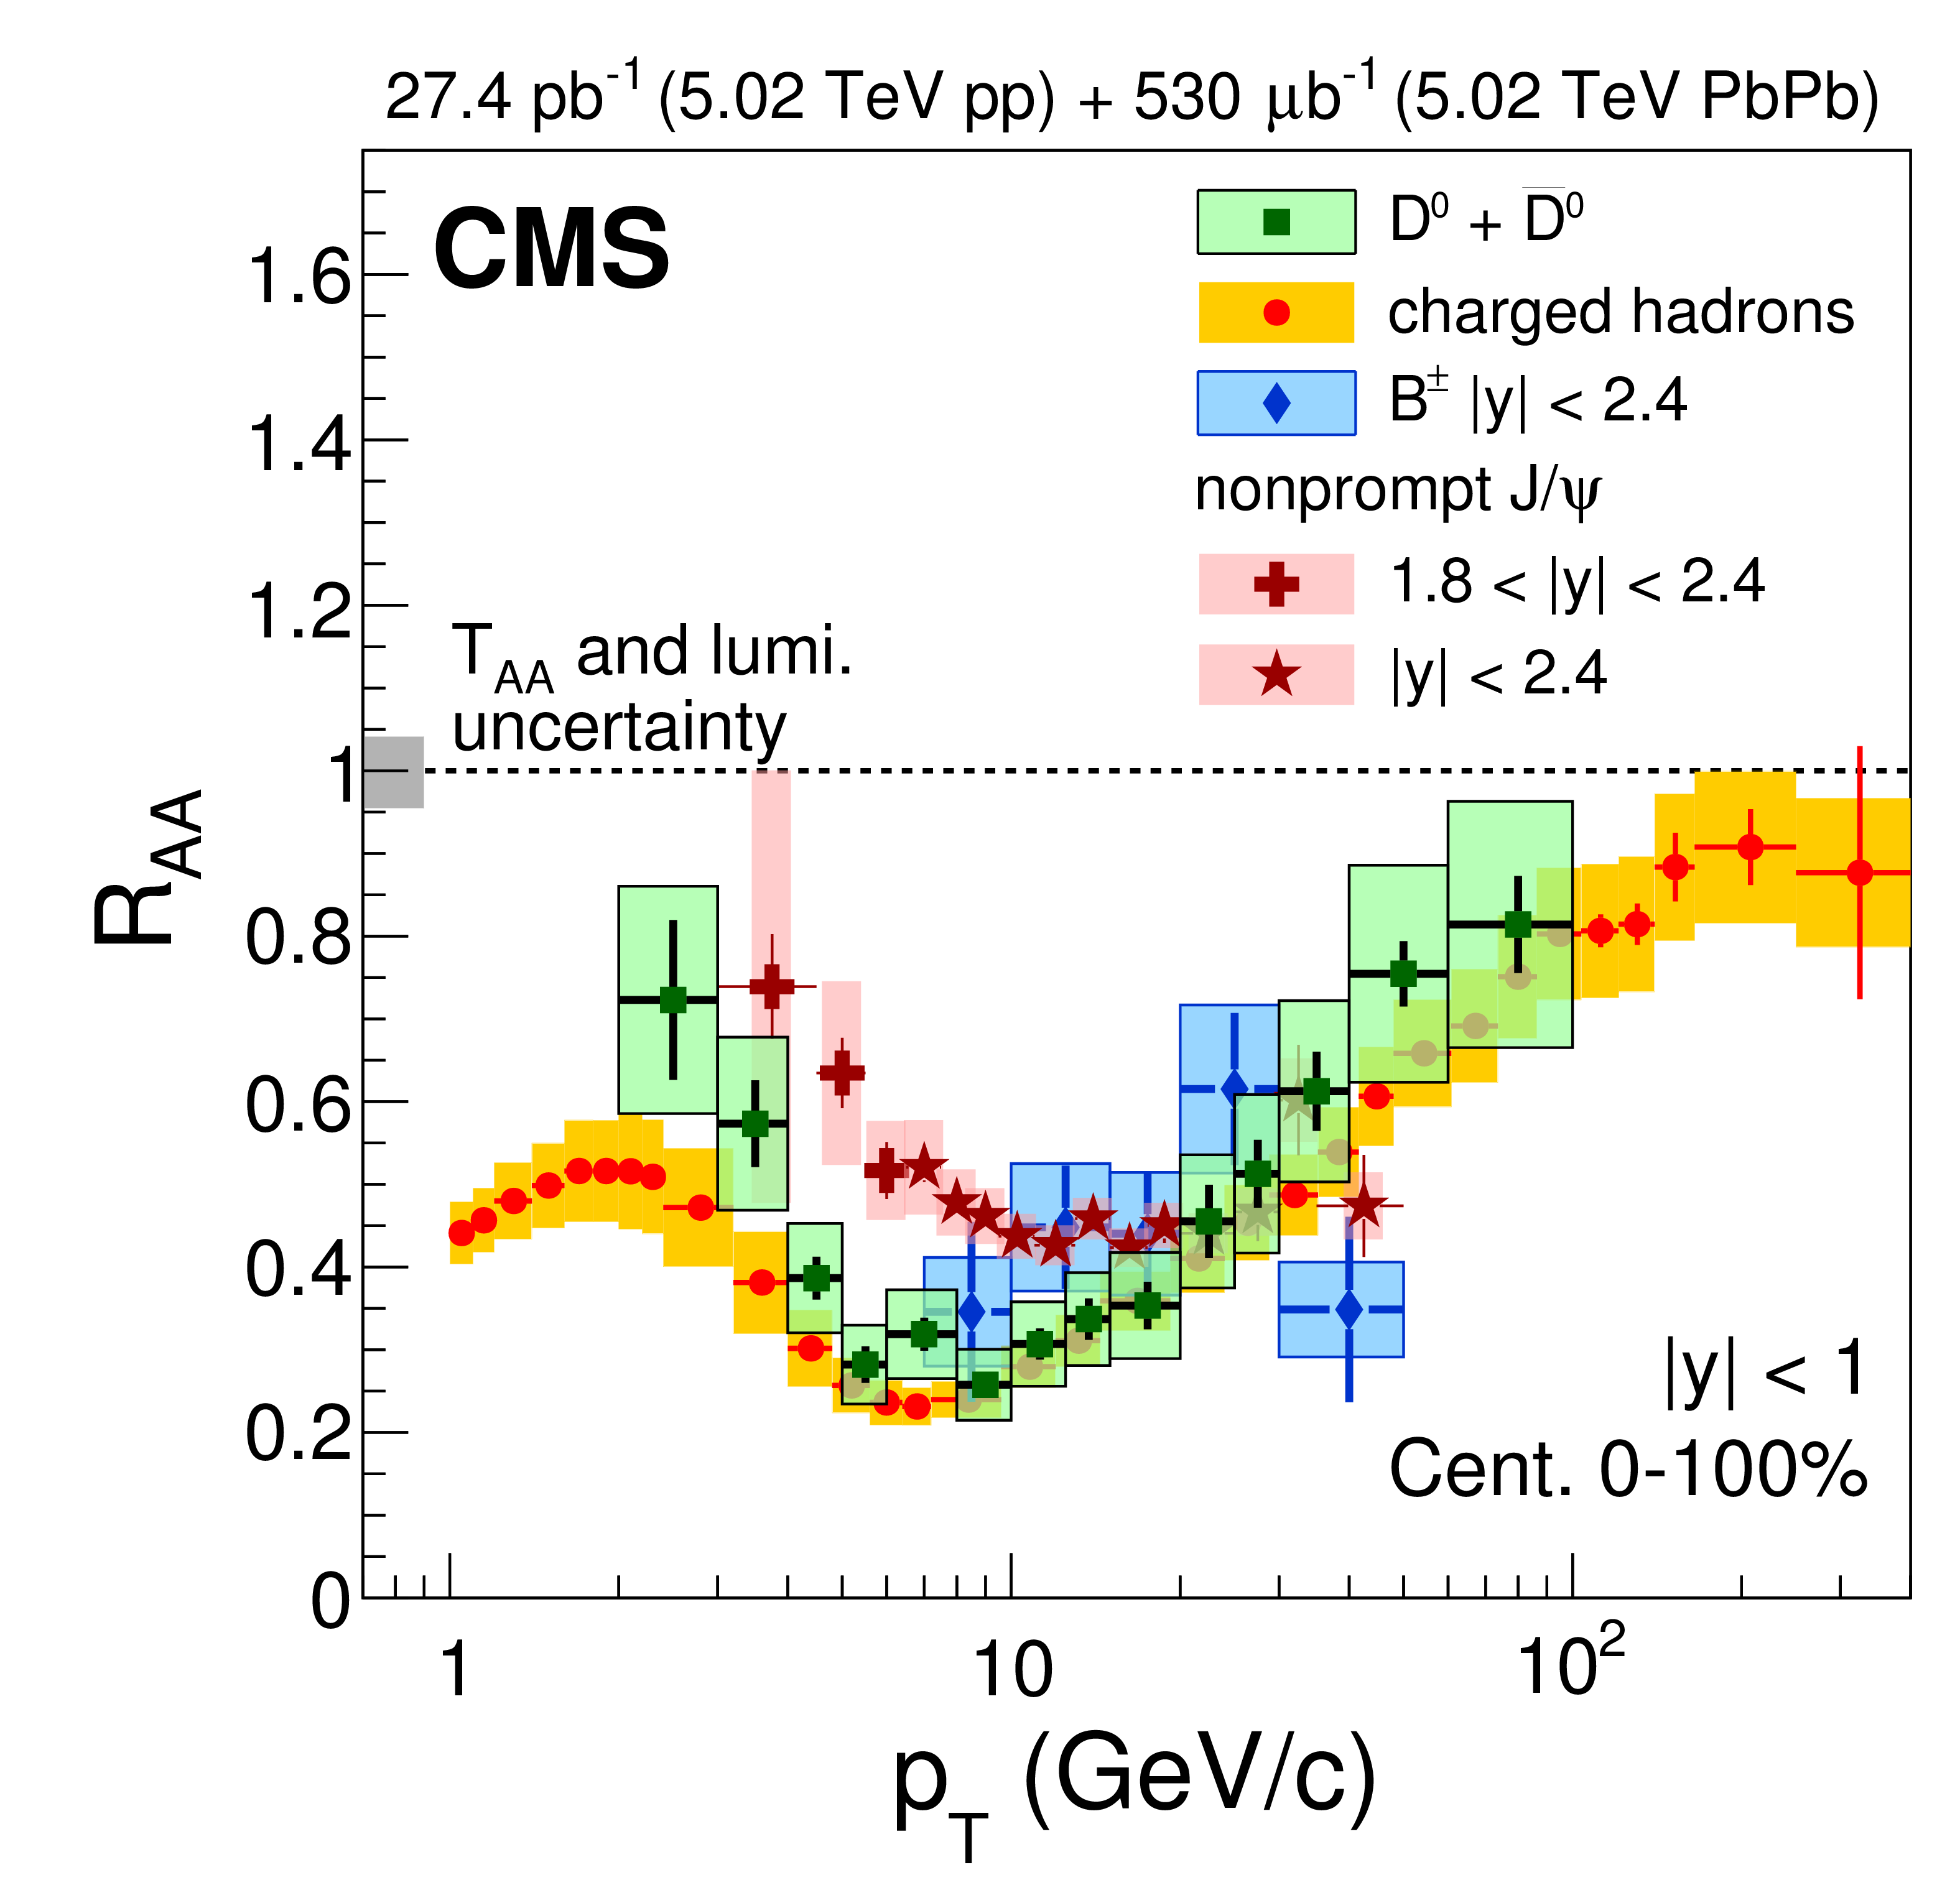
\includegraphics[width=0.47\textwidth]{Figures/Chapter2/CMSRAA.png}
\caption{The fully reconstructed $D^0$ $R_{AA}$ vs $p_T$ with the STAR experiment in 0 - 10\%, 10 - 40\%, and 40 - 80\% centrality at RHIC and $D^0$, $B^+$, non-prompt $J/\psi$, and charged hadrons $R_{AA}$ vs $p_T$ at 0 - 100\% centrality with the CMS experiment at LHC are shown above.}
\label{HQRAA}
\end{center}
\end{figure}   

We could see that the $R_{AA}$ of $D^0$ and $B^+$ are both below 1, which suggests charm and beauty quarks lose a significant fraction of energy to the QGP medium. As $p_T$ increases, the $R_{AA}$ of light and heavy flavor hadrons converge to the same values and approach unity where Lorentz $\gamma$ factor comes into play and the mass of the hadron becomes irrelevant. In addition, the CMS results above indirectly agree with the expectation of the flavor dependence of energy loss: $R_{AA}^{h} < R_{AA}^{D} < R_{AA}^{B} < 1$. Most theoretical model calculations are in reasonable agreement with the $R_{AA}$ data. 

To better constrain theoretical model calculations and understand the energy loss mechanism of heavy quarks in the QGP medium, we need to perform more precise measurements of B- and D-mesons $R_{AA}$ and $v_2$ down to lower $p_T$ where the mass of heavy quarks becomes important and models diverge from each other. The ALICE experiment has performed the first measurement of prompt and non-prompt $D^0$ $R_{AA}$ down to $p_T =$ 0 shown in Figure \ref{ALICEDRAALow} below


\begin{figure}[hbtp]
\begin{center}
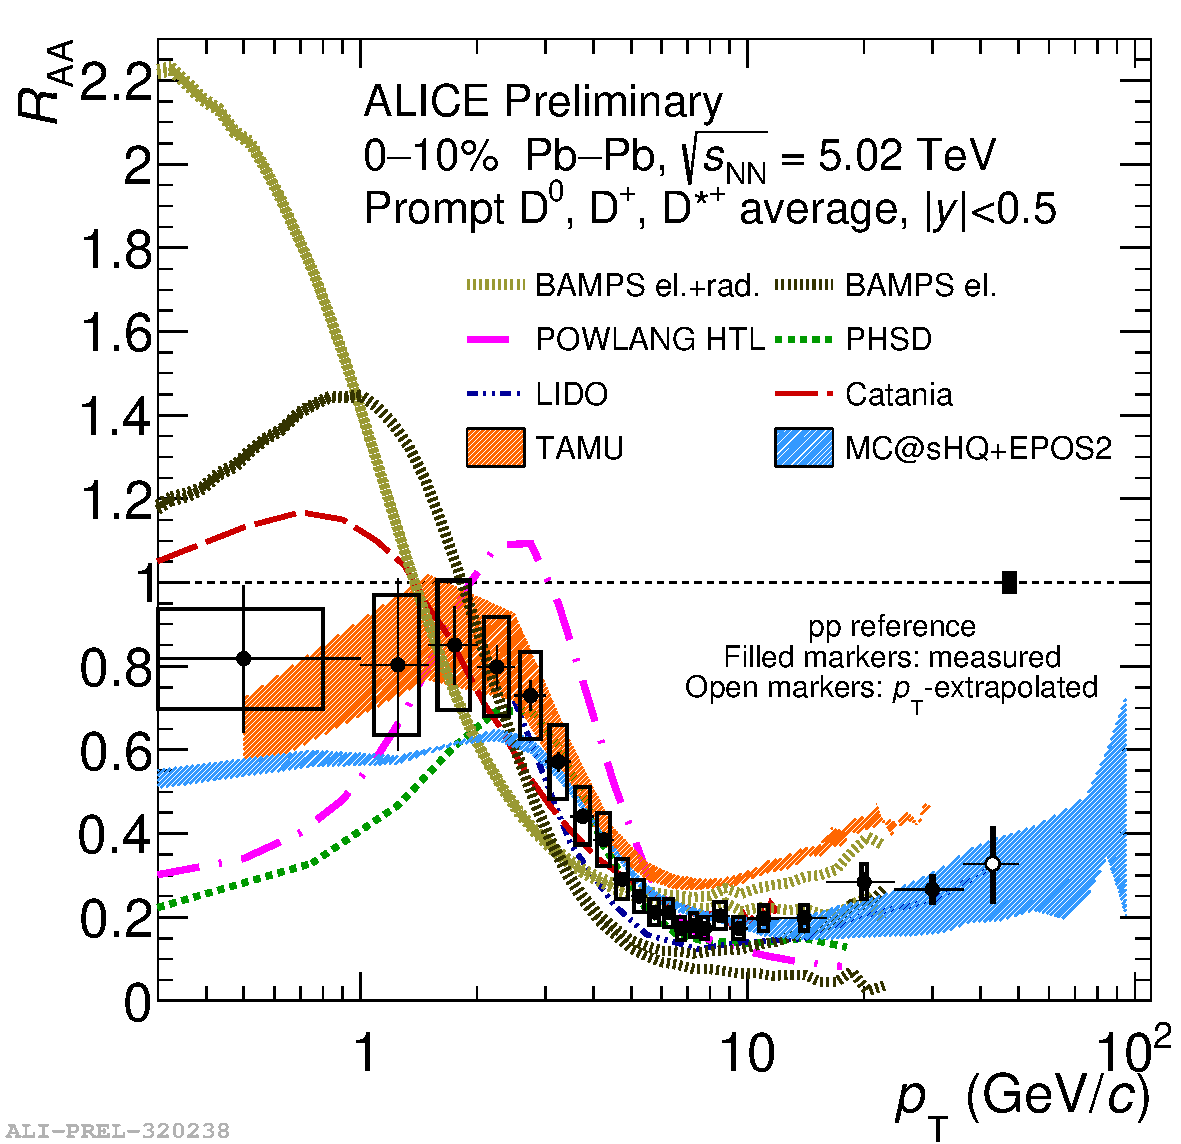
\includegraphics[width=0.48\textwidth]{Figures/Chapter2/ALICEDRAALow.pdf}
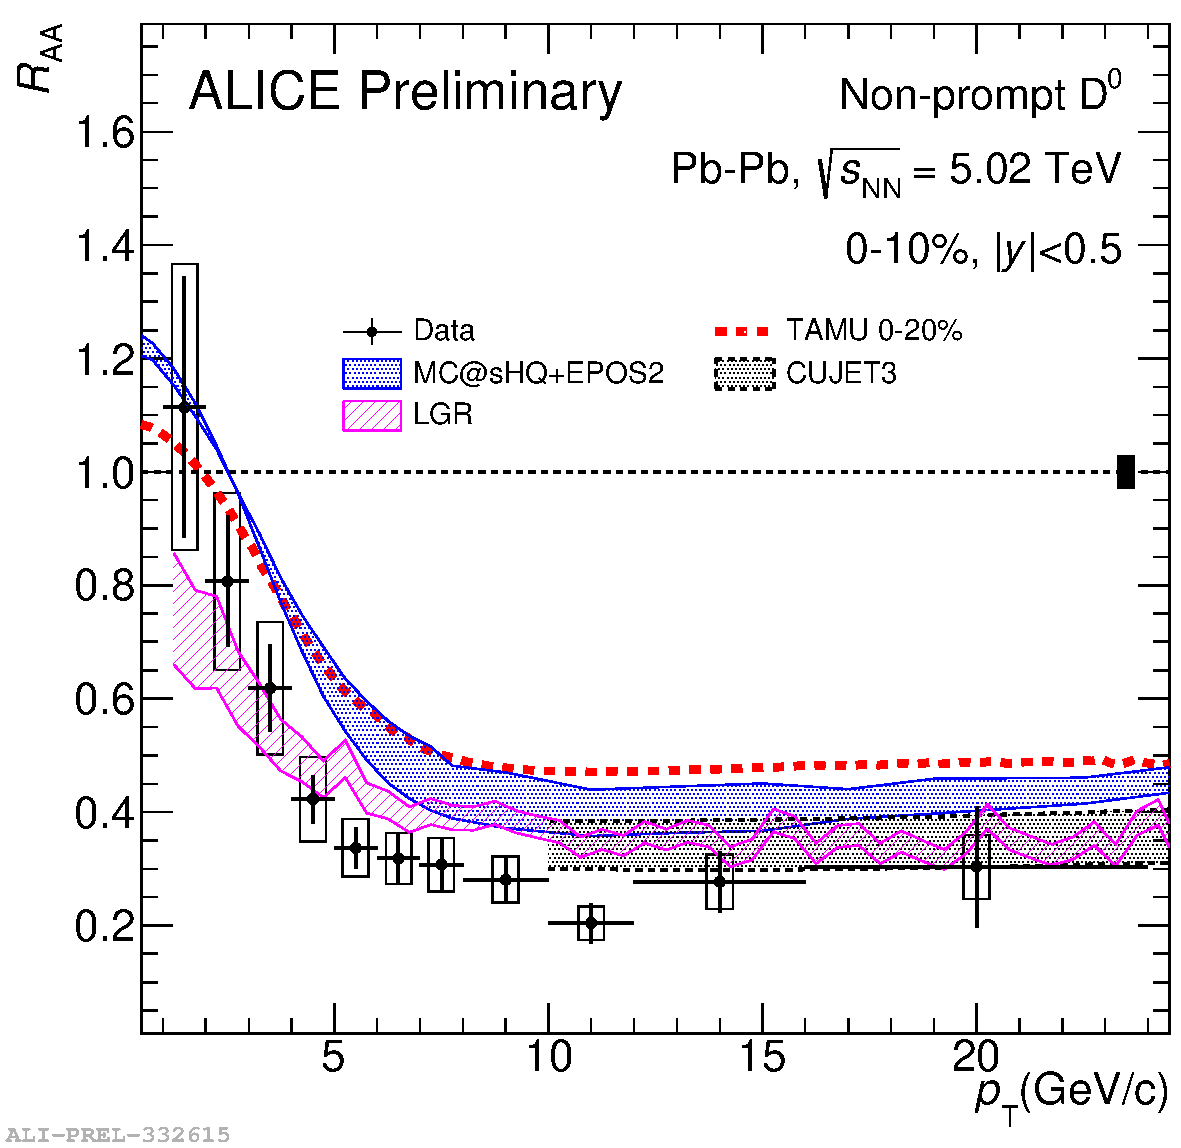
\includegraphics[width=0.48\textwidth]{Figures/Chapter2/ALICENPDRAALow.pdf}
\caption{The $R_{AA}$ of prompt D mesons vs $p_T$ down to $p_T$ = 0 (left) and non-prompt D mesons down to $p_T$ = 1 GeV/c (right) are shown above.}
\label{ALICEDRAALow}
\end{center}
\end{figure}   

From the ALICE measurement of prompt and non-prompt D mesons $R_{AA}$ down to very low $p_T$, we could see that very few models are able to simultaneously describe $D^0$ $R_{AA}$ at both low and high $p_T$. Nonetheless, the fully reconstructed B-meson $R_{AA}$ measurement from exclusive b decay down to very low $p_T$ is still missing. We should try to perform B-meson $R_{AA}$ measurement down to very low $p_T$ to provide a complete picture to constrain the jet transport coefficient $\hat q$ and heavy-quark diffusion coefficient. Also, fully reconstructing B mesons down to $p_T$ = 0 will allow us to measure inclusive beauty production cross section in $pp$ collisions and test pQCD calculations.  


\section{Production Yield Ratio}

According to the theoretical reviews of heavy-quark hadrochemistry in heavy-ion collisions \cite{StrangetoLight,BaryontoMeson}, the strange-to-non-strange meson ($H_s/H^0$) and baryon-to-meson ($\Lambda_{Q}/H^{0}$) ratios are excellent observables to test hadronization models. Both RHIC and LHC have carried out extensive measurements of fully reconstructed charm hadron yield ratios. Figure \ref{HadroPlotCharm} shows the fully reconstructed prompt $D^+_s/D^0$ ratios measured by the STAR \cite{STARDsD0Ref} and ALICE \cite{ALICEDsD0Ref} experiments


\begin{figure}[hbtp]
\begin{center}
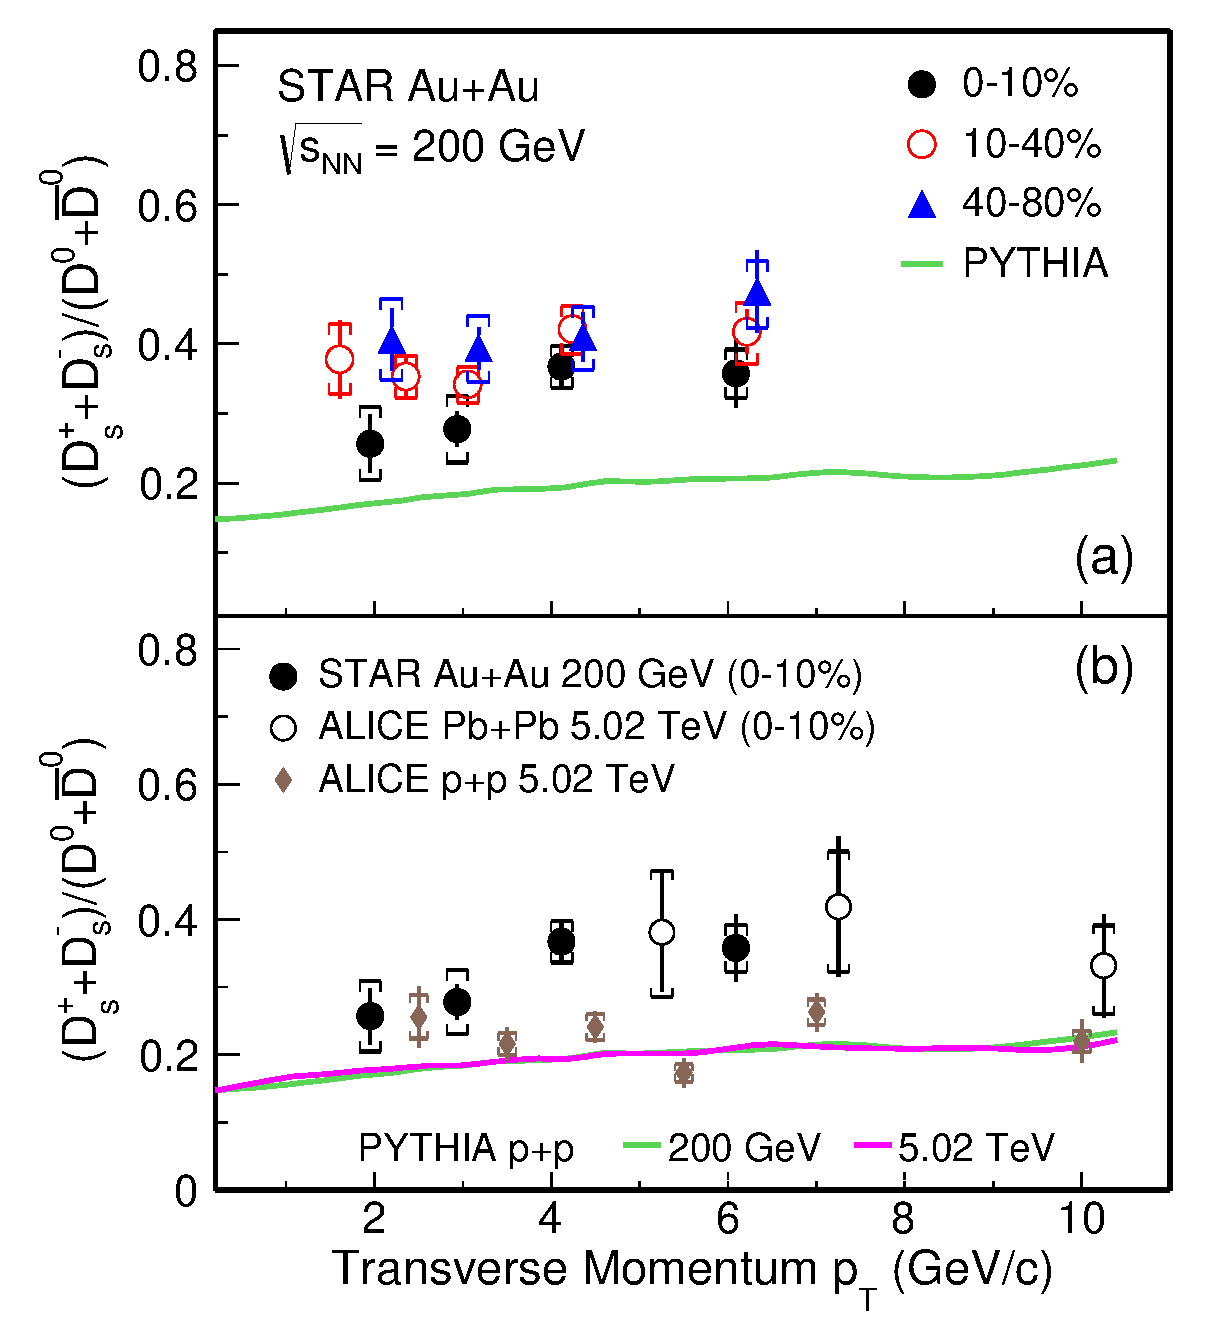
\includegraphics[width=0.45\textwidth]{Figures/Chapter2/STARDsD0.eps}
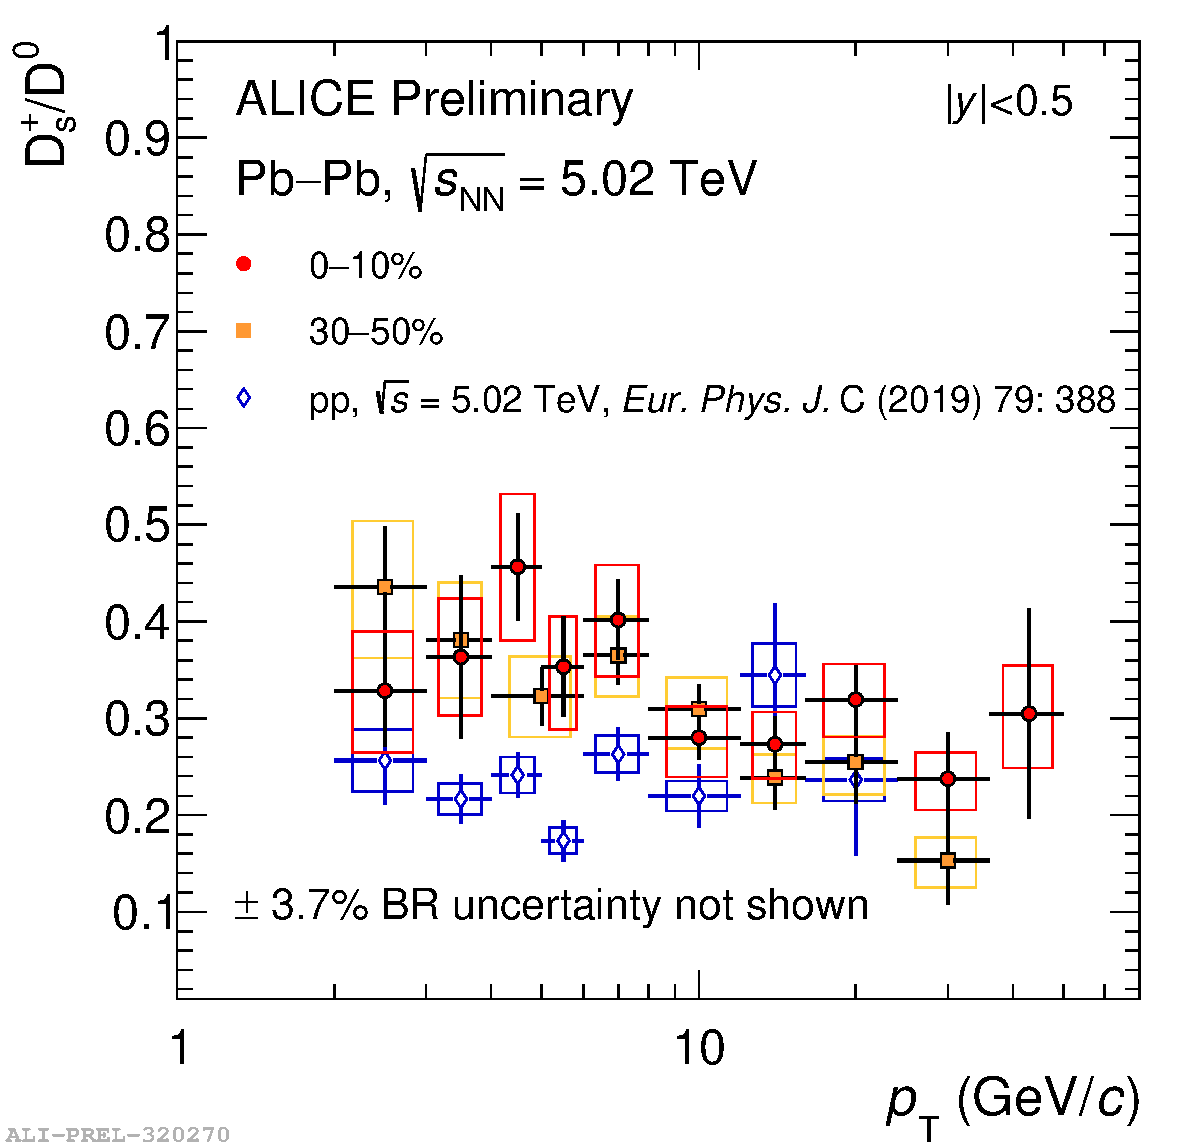
\includegraphics[width=0.51\textwidth]{Figures/Chapter2/ALICEDsD0.pdf}
\caption{The fully reconstructed $D_s^+/D^0$ ratios in Au + Au measured by the STAR experiment at RHIC (left) and in PbPb the ALICE experiment at LHC (right) as functions of $p_T$ are shown above.}
\label{HadroPlotCharm}
\end{center}
\end{figure}   


We can see that in general, both $D_s^+/D^0$ ratios in heavy-ion collisions lie above $pp$ collisions.

Figure \ref{HadroPlotCharm} shows the fully reconstructed $\Lambda_c^+/D^0$ ratios measured by the STAR \cite{STARLambdaCD0} and ALICE \cite{ALICELambdaCD0} experiments



\begin{figure}[hbtp]
\begin{center}
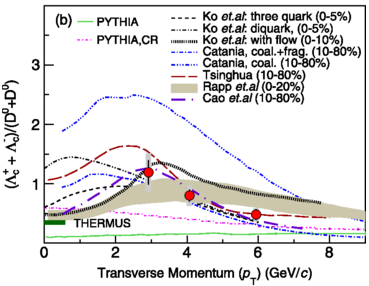
\includegraphics[width=0.48\textwidth]{Figures/Chapter2/STARLambdaCD0.png}
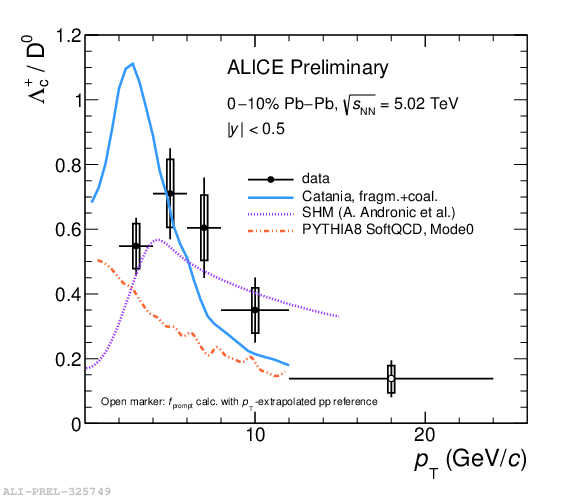
\includegraphics[width=0.48\textwidth]{Figures/Chapter2/ALICELambdaCD0}
\caption{The fully reconstructed $\Lambda_c^+/D^0$ ratio in $pp$ and heavy-ion collisions measured by the STAR experiment at RHIC (left) and the CMS experiment at LHC (right) are shown above.}
\label{HadroPlotCharm}
\end{center}
\end{figure}   



Many different theoretical predictions agree reasonably well with the experiments due to their large uncertainties. However, these large discrepancies among hadronization models significantly limit our ability to interpret heavy flavor experimental data. 

The ALICE experiment also performs a comprehensive study on charm quark hadronization in $pp$, pPb, and PbPb. Figure \ref{ALICEMulti} shows the $D^+_s/D^0$ and $\Lambda_c/D^0$ ratios as functions of event multiplicity from small to large collision systems. 

\begin{figure}[hbtp]
\begin{center}
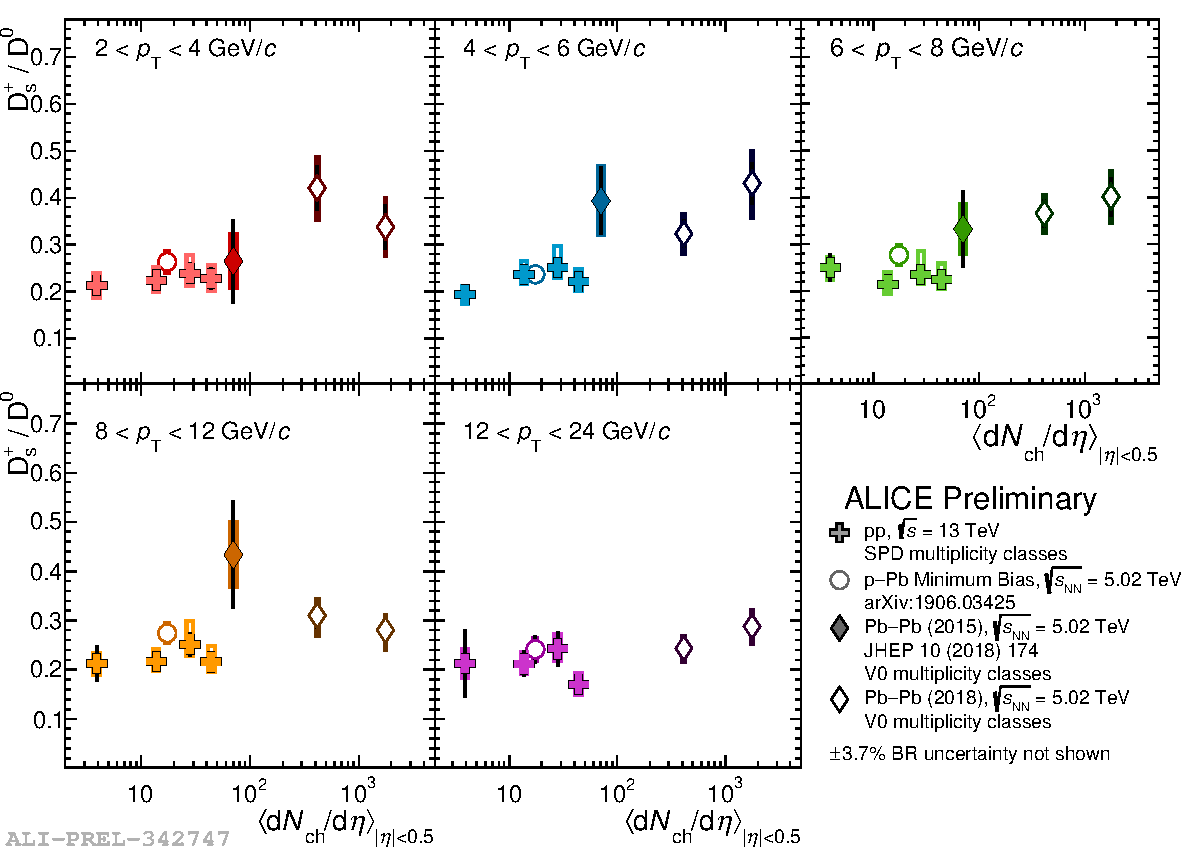
\includegraphics[width=0.80\textwidth]{Figures/Chapter2/ALICEDsD0Multi.pdf}
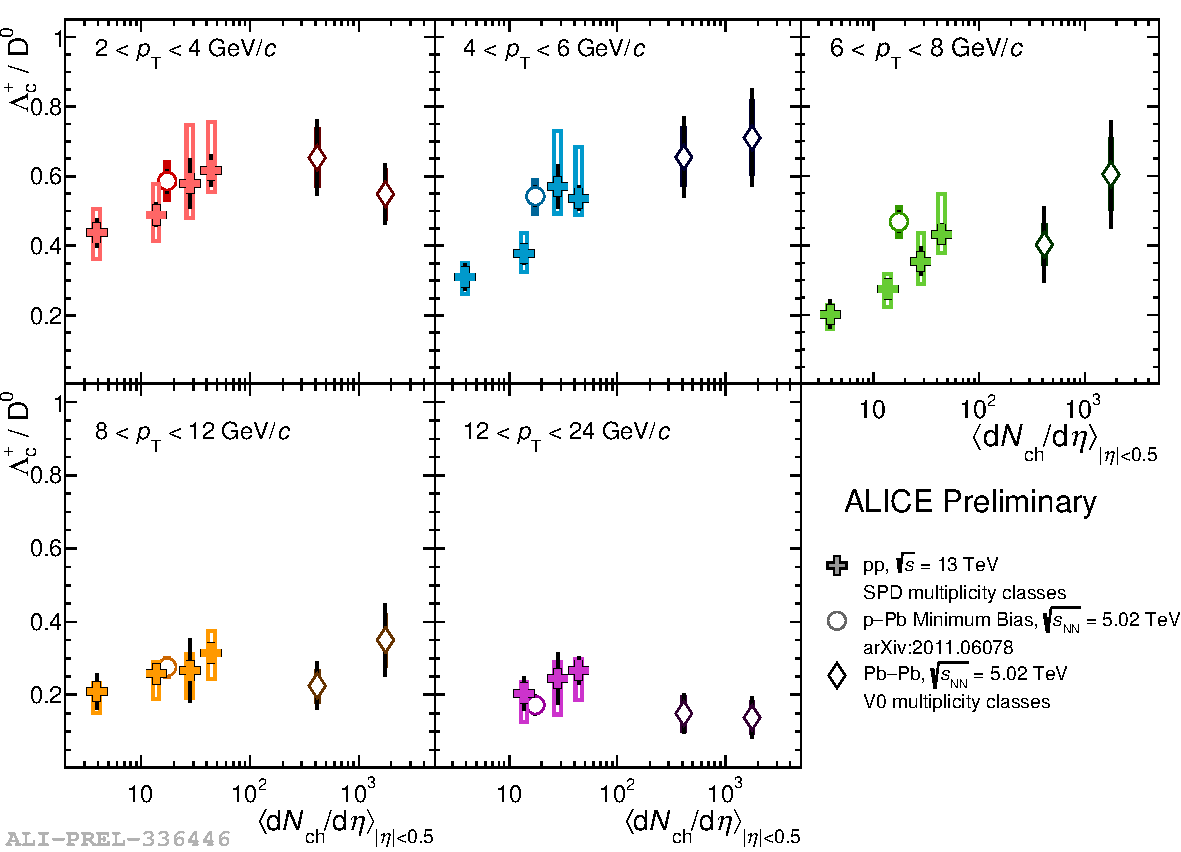
\includegraphics[width=0.80\textwidth]{Figures/Chapter2/ALICELambdaD0Multi.pdf}
\caption{The fully reconstructed $D^+_s/D^0$ (top) and $\Lambda_c^+/D^0$ ratios (bottom) as a function of event multiplicity $\langle dN_{ch}/d\eta \rangle$ within $|\eta| < 0.5$ in $p_T$ from 2 - 4, 4 - 6, 6 - 8, 8 - 12, and 12 - 24 GeV/c in $pp$, pPb, and PbPb collisions measured by the ALICE experiment are shown above.}
\label{ALICEMulti}
\end{center}
\end{figure}   



In the multiplicity studies, overall increasing trends of both $D^0_s/D^0$ and $\Lambda_c^+/D^0$ ratios in higher multiplicity are observed. Moreover, this is only in the charm sector. Similar fully reconstructed b-hadron measurements to study beauty hadrochemistry are still missing. 


%Bs/B+

\clearpage

Therefore, it is crucial to have more precise measurements over a wide range of $p_T$ and multiplicity in both beauty and charm sectors to constrain theoretical models. Currently, the only published fully reconstructed b-hadron measurements in heavy-ion collision are the $B^0_s$ and $B^+$ based on CMS 2015 PbPb datasets \cite{CMSBsBP2015}. Figure \ref{BsBP2015} shows the $B^0_s$ $B^+$ $R_{AA}$ $R_{AA}$ and their ratios in $pp$ and PbPb collisions

\begin{figure}[hbtp]
\begin{center}
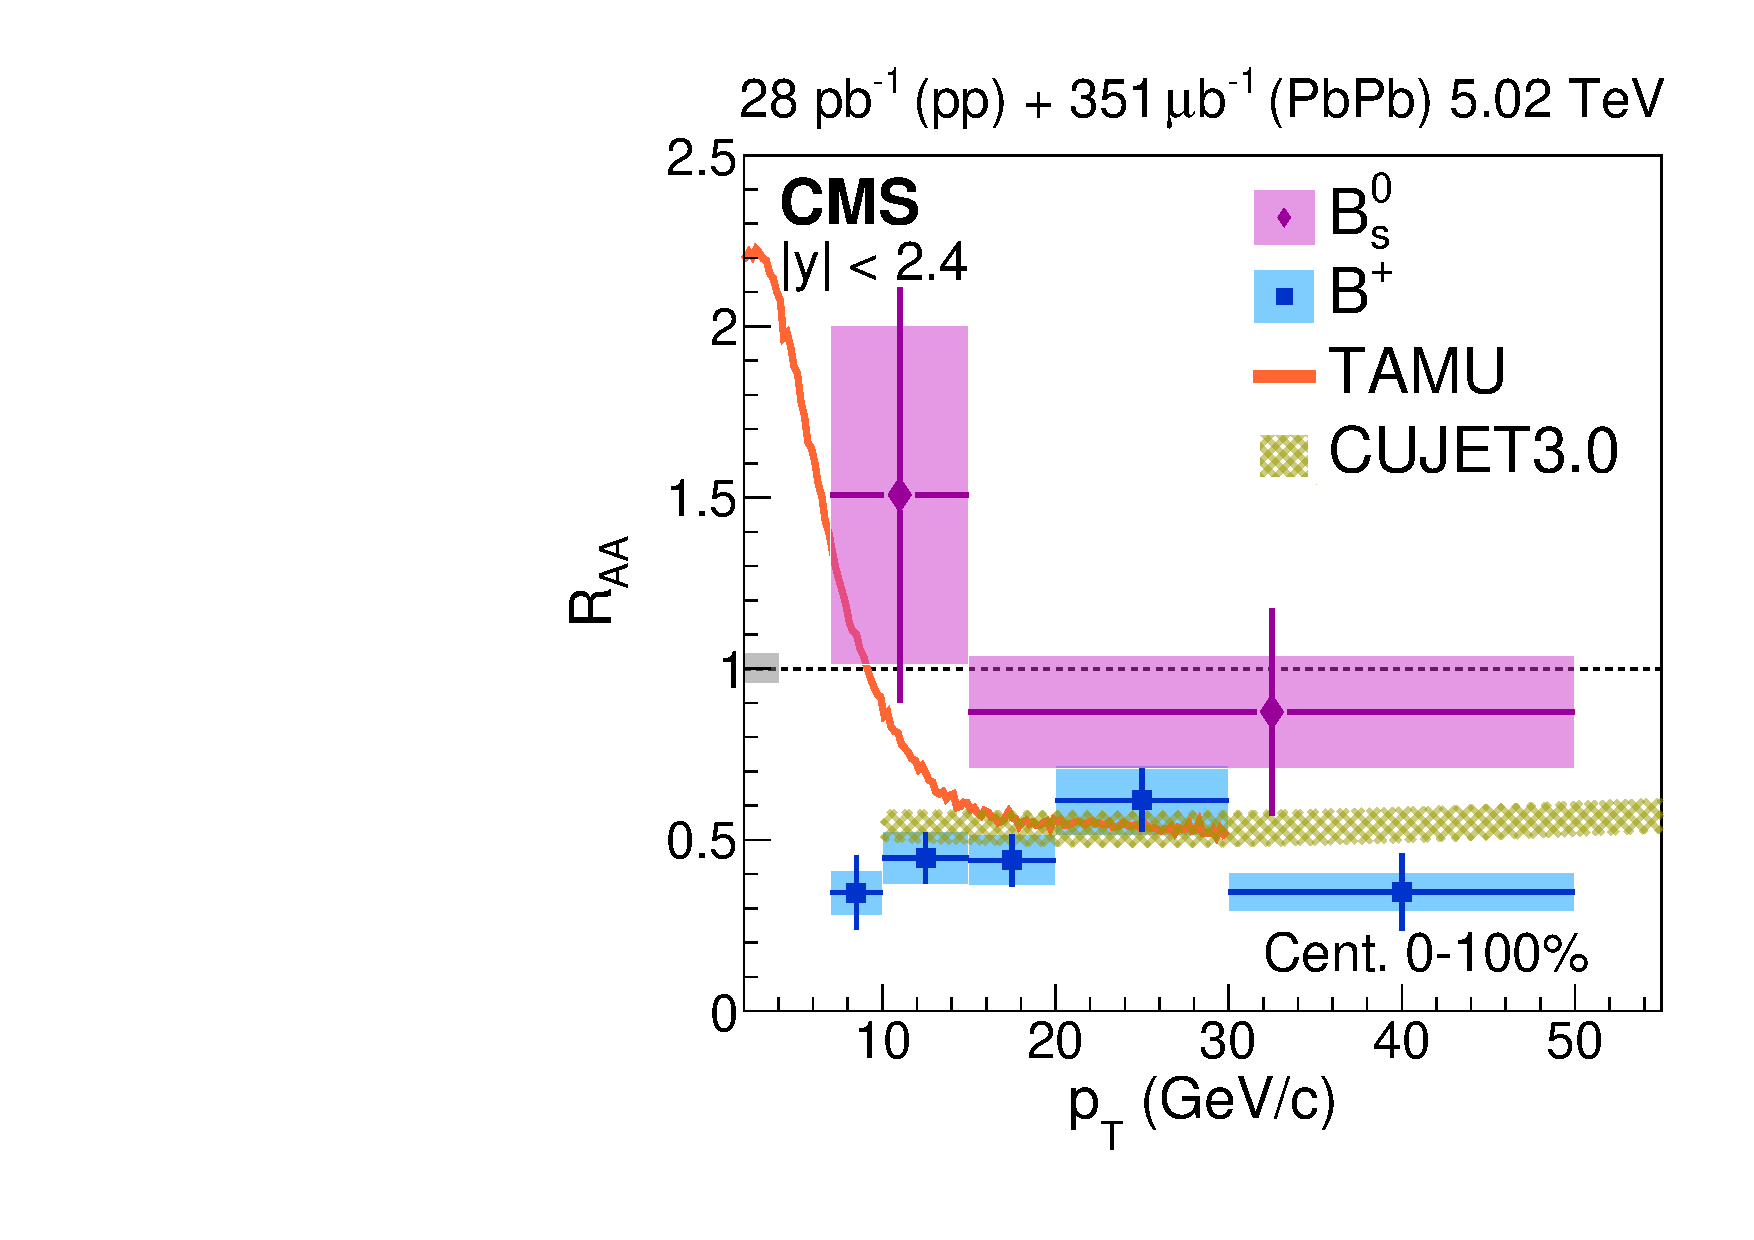
\includegraphics[width=0.48\textwidth]{Figures/Chapter2/CMSBsBPRAA2015.pdf}
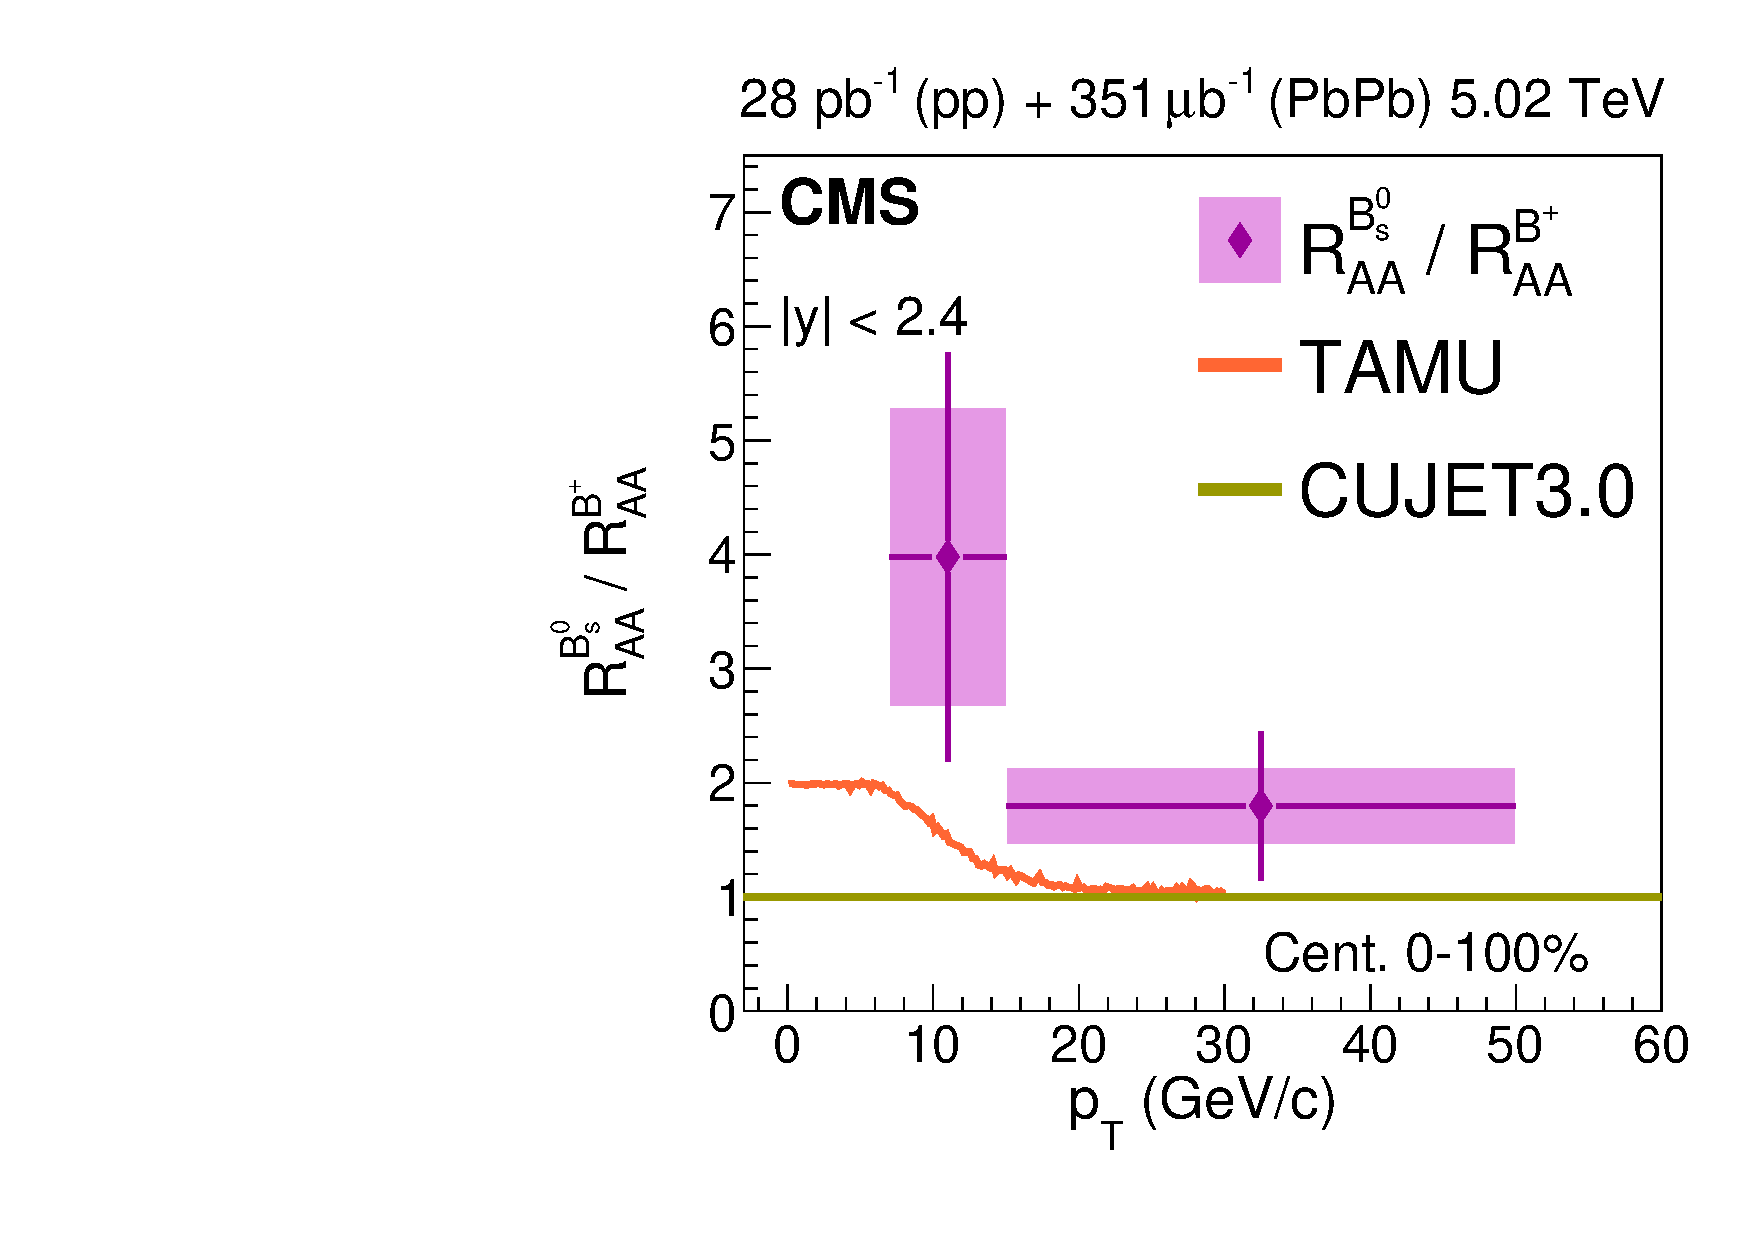
\includegraphics[width=0.48\textwidth]{Figures/Chapter2/CMSBsBP2015.pdf}
\caption{The fully reconstructed $B^0_s$ and $B^+$ $R_{AA}$ (left) and $B^0_s/B^+$ $R_{AA}$ ratio (right) as a function of $p_T$ using the 2015 CMS $pp$ and PbPb datasets are shown above.}
\label{BsBP2015}
\end{center}
\end{figure}   


These first fully reconstructed B-meson measurements in heavy-ion collisions are good. Nonetheless, the $B^0_s$ measurement has relatively large uncertainties due to the very limited statistics. The $B^0_s$ significance is still below 5$\sigma$. In order to better constrain hadronization model calculations and better interpret our data, we should perform more differential measurements in the beauty sector with enhanced precision. 

In the baryon-to-meson ratio studies, LHCb has conducted fully reconstructed $\Lambda_b^0/B^+$ ratio in $pp$ and pPb collision \cite{LHCbLambdaB} shown below in Figure \ref{LHCbLambda}


\begin{figure}[hbtp]
\begin{center}
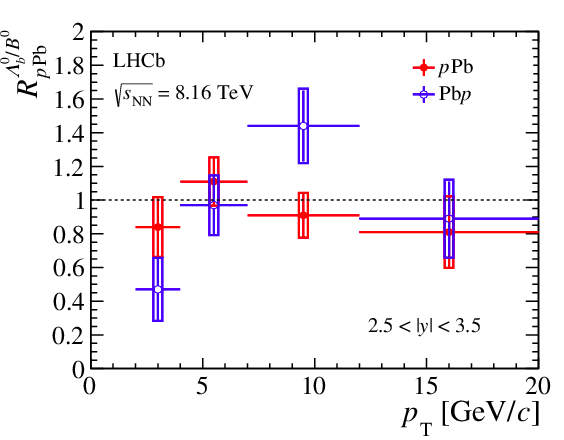
\includegraphics[width=0.48\textwidth]{Figures/Chapter2/LHCbRpAPt.png}
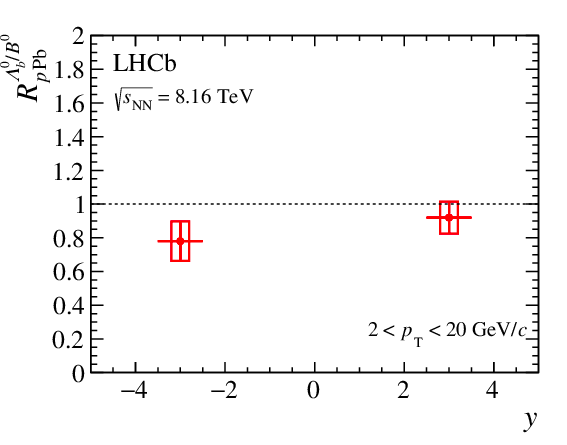
\includegraphics[width=0.48\textwidth]{Figures/Chapter2/LHCbRpAy.png}
\caption{The fully reconstructed $\Lambda_b^0/B^+$ $R_{pA}$ ratios as a function $p_T$ (left) and $y$ (right) in $pp$, pPb, and Pbp collisions measured by the LHCb experiment are shown above.}
\label{LHCbLambda}
\end{center}
\end{figure}   

The $\Lambda_b^0/B^0$ double ratios in pPb to $pp$ in the forward region are near unity according to the LHCb measurement. No significant $p_T$ or $y$ dependence is observed. It would be interesting to conduct similar measurements in mid-rapidity region in $pp$ and pPb collisions. However, so far no fully reconstructed $\Lambda_b^0$ measurement has been carried out in heavy-ion collisions due to the limited statistics and large combinatorial background of $\Lambda_b^0$. 



\section{Heavy Flavor Hadron-Jet Angular Correlations}

Aside from the traditional heavy flavor observables: $R_{AA}$, $v_{2}$, and production yield ratio, modern observables, such as heavy flavor hadron-hadron and heavy flavor hadron-jet angular correlations, have better differentiation to provide more insight for the understanding of the dynamics and interaction mechanism of heavy quarks in the QGP medium. 

The measurements of angular correlations between heavy flavor hadrons and jets can be used to constrain parton energy loss mechanisms and to better understand heavy-quark diffusion in the medium. From the D-jet angular correlation studies, the quantitive studies of the medium modification to the radial profile of charm quarks could shed light on the interaction mechanism of charm quarks with the medium. Figure \ref{DJETCorr} shows the measurement of D-jet angular correlation in PbPb and $pp$ collisions with the CMS experiment \cite{CMSDJet}

\begin{figure}[hbtp]
\begin{center}
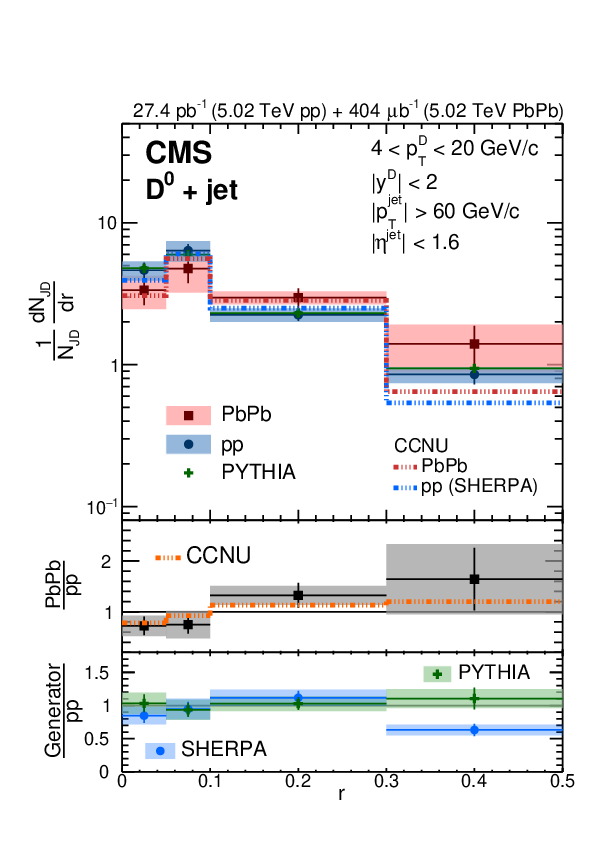
\includegraphics[width=0.48\textwidth]{Figures/Chapter2/CMSDJetLow.png}
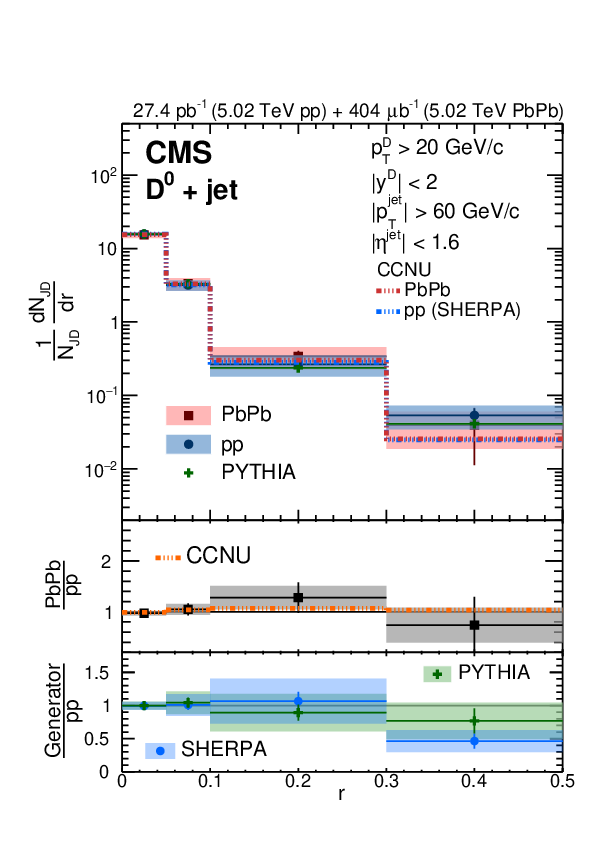
\includegraphics[width=0.48\textwidth]{Figures/Chapter2/CMSDJetHigh.png}
\caption{Distributions of fully reconstructed $D^0$ mesons in jets, as a function of the distance from the jet axis ($r$) for jets of $p_T^{jet} >$ 60 GeV/c and $|\eta^{jet}| <$ 1.6 measured in $pp$ and PbPb collisions at $\sqrt{s_{NN}} = $ 5.02 TeV, for $4 < p_T^D < 20$ GeV/c and $p_T^D > 20$ GeV/c, are shown above. The jet radius is defined as $r = \sqrt{(\Delta \phi_{jD})^2 +  (\Delta \eta_{jD})^2 }$ where $\phi_{jD}$ and $\eta_{jD}$ are the $\eta$ and $\phi$ of the $D^0$ meson with respect to the jet axis.}
\label{DJETCorr}
\end{center}
\end{figure}   

At low $p_T$, the $D^0$ mesons are pushed radially outward in PbPb collisions compared to $pp$, which shows effects of charm-quark diffusion with the presence of the QGP medium. At high $p_T$, the shape is approximately consistent with unity. While the CCNU model is in reasonably good agreement with the PbPb/$pp$ ratio, its predictions are lower compared to the measurements of $\frac{1}{N_{jD}}\frac{dN_{jD}}{dr}$ in individual $pp$ and PbPb collisions.


\section{Heavy Flavor Hadron-Hadron Correlations}

Another observable is heavy flavor hadron-hadron correlation, which is even better to tag the heavy quark $Q\bar Q$ pair the produced back-to-back in the early stage of hard scattering processes and understand the modification effects as they propagate through vacuum and medium. Experimentally, the observable is a fully reconstructed open heavy flavor hadron correlates with associated hadrons produced within the same event and subtracts the background in mixed events. In the analysis, $\Delta \eta$ and $\Delta \phi$ distributions of the heavy flavor hadrons from associated hadrons are used to quantify the correlation. Figure \ref{ALICEDHadron} shows the D meson-hadron angular correlation measured with the ALICE experiment \cite{DHadronRef}


\begin{figure}[hbtp]
\begin{center}
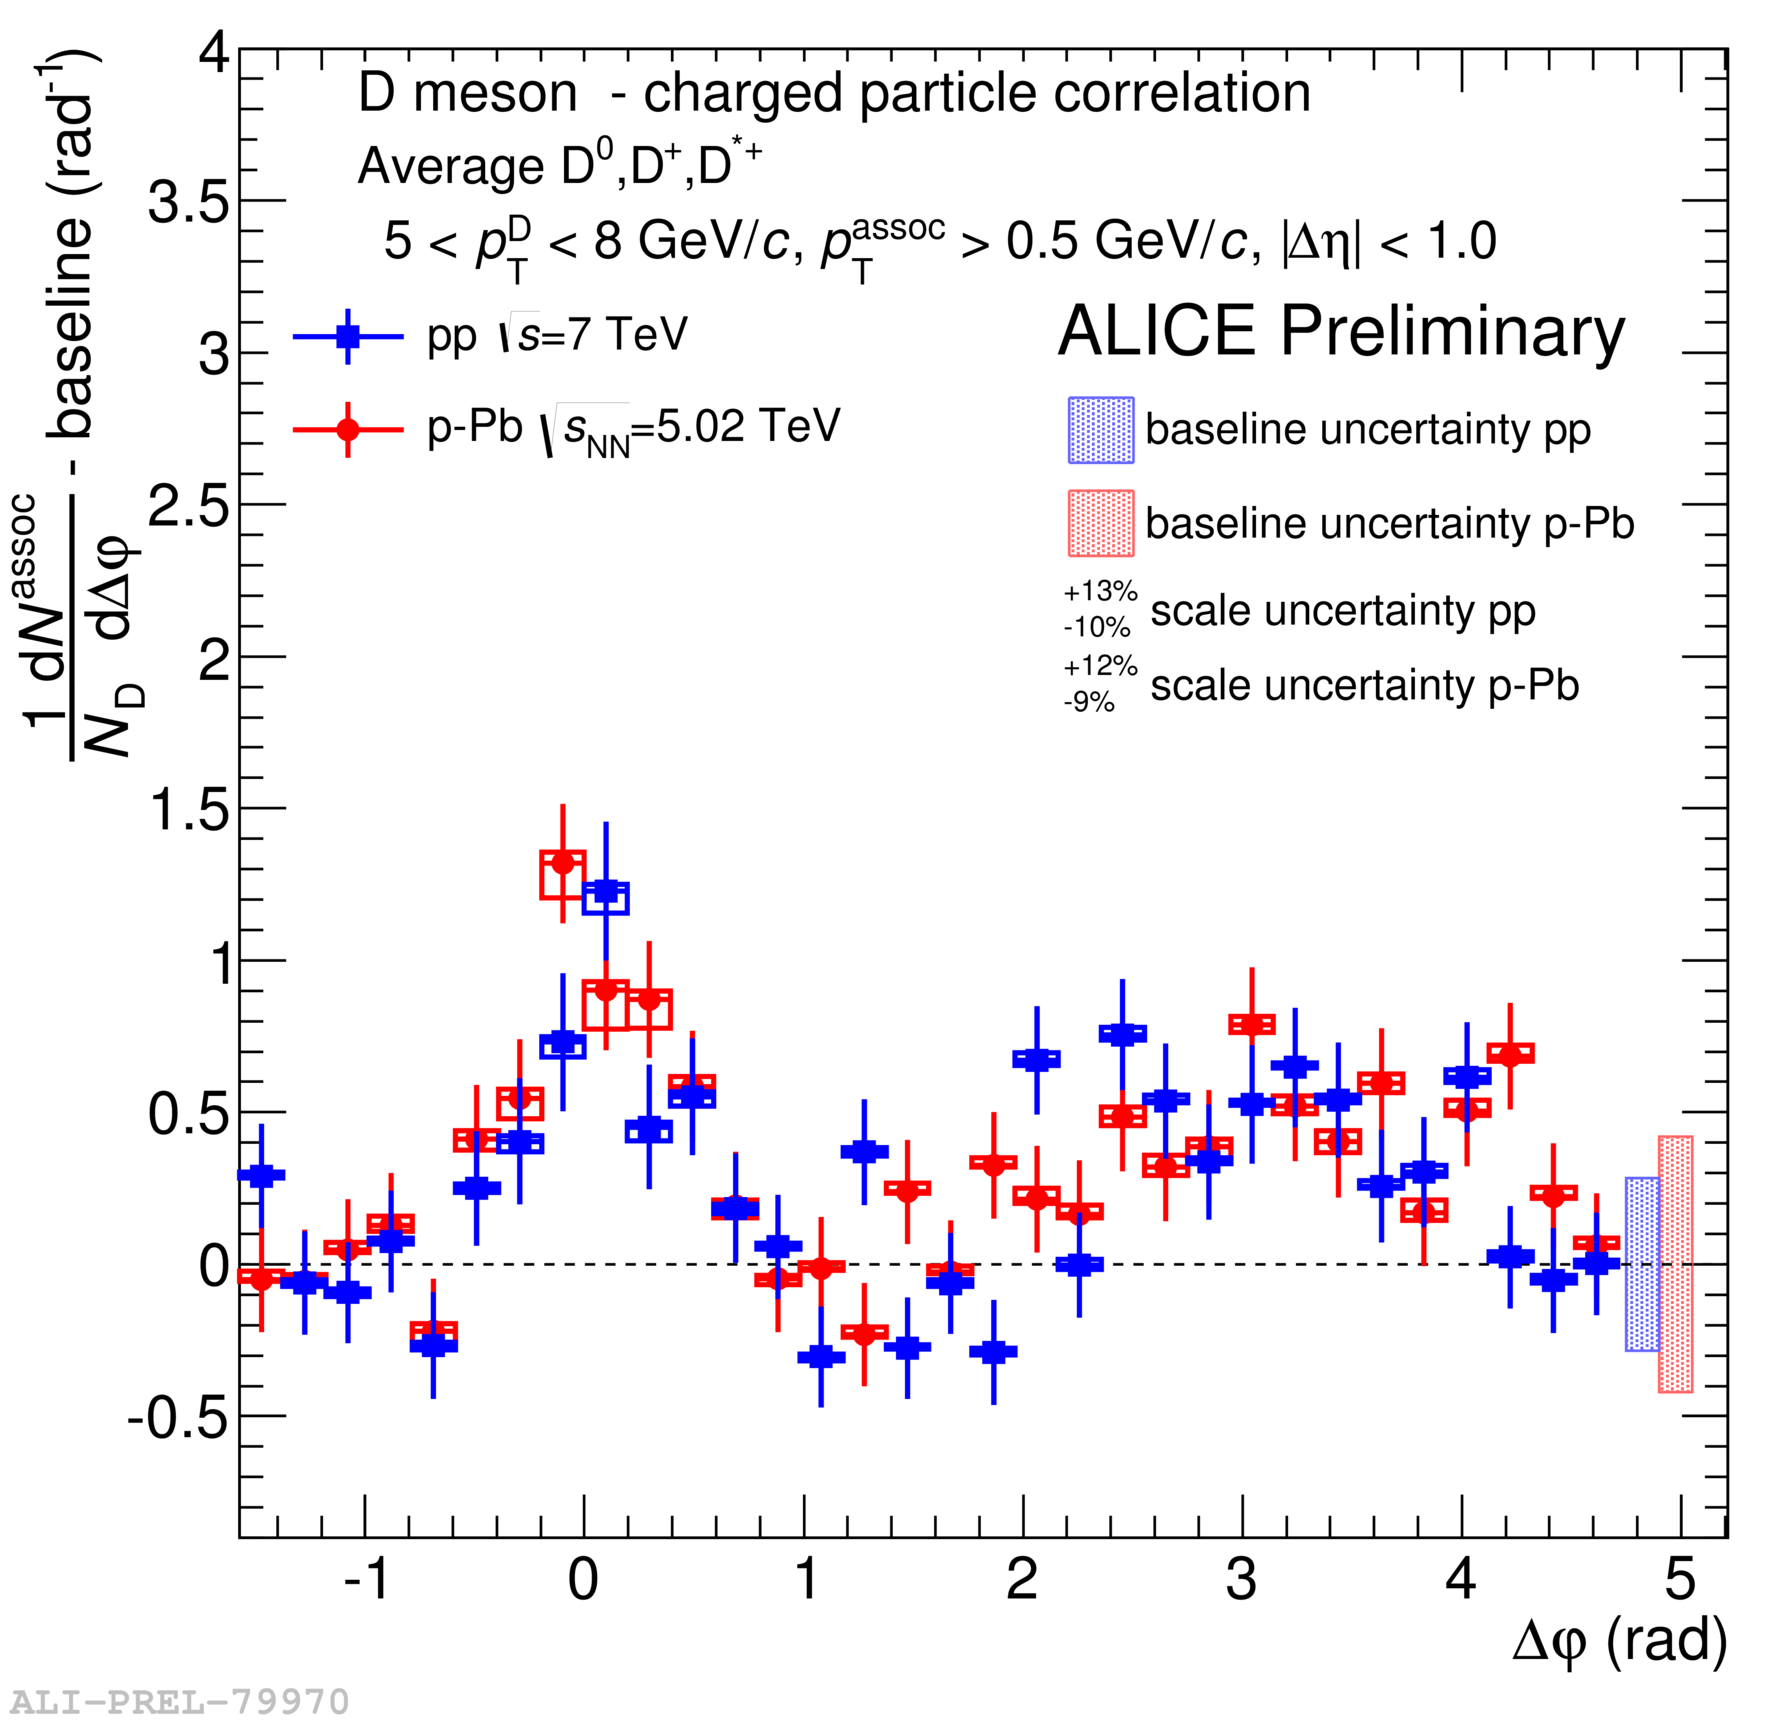
\includegraphics[width=0.48\textwidth]{Figures/Chapter2/ALICEDHadron.png}
\includegraphics[width=0.48\textwidth]{Figures/Chapter2/ALICEDHadronPP.png}
\caption{The ALICE D-hadron angular correlation in both $pp$ (blue) and pPb (red) collision (left) and the comparison of $pp$ data with PYTHIA calculations (right) are shown above.}
\label{ALICEDHadron}
\end{center}
\end{figure}   

In the D-hadron correlation, there are two peaks at $\Delta \phi =$ 0 and $\pi$. At $\Delta \phi = $0, hadrons are produced along with the charm quarks via fragmentation mechanism. At $\Delta \phi = \pi$, the hadrons are produced from back-to-back jets to maintain momentum conservation. The $pp$ measurements are overall consistent with PYTHIA calculations. From the comparison between the results in the $pp$ and pPb, the D-hadron angular correlation distributions are compatible with each other within uncertainties. Consequently, no evident effects on the charm fragmentation and hadronization due to cold nuclear matter can be claimed  \cite{DHadronRef}. 

STAR has also performed the 2D $\Delta \eta \times \Delta \phi$ measurement of fully reconstructed $D^0$-hadron correlation in Au + Au collisions \cite{DHadronSTAR} shown in Figure \ref{STARDHadron}

\begin{figure}[hbtp]
\begin{center}
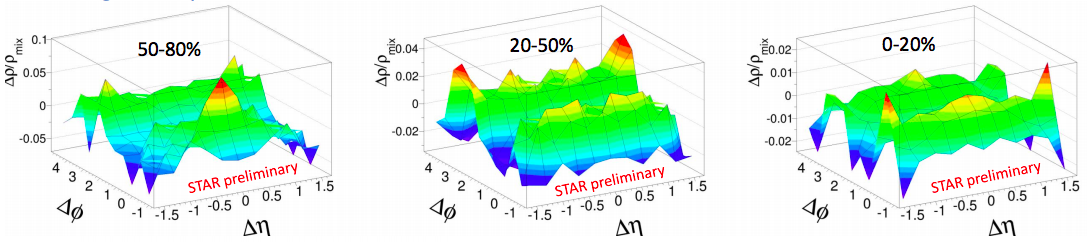
\includegraphics[width=1.05\textwidth]{Figures/Chapter2/STARDHadron.png}
\caption{The 2D $\Delta \eta \times \Delta \phi$ distributions of $D^0$ mesons and associated hadrons in Au + Au centrality 0 - 20\%, 20 - 50\%, and 50 - 80\% at $\sqrt{s_{NN}} = $ 200 GeV measured by the STAR experiment are shown above.}
\label{STARDHadron}
\end{center}
\end{figure} 

As expected, the $D^0$-hadron angular correlation get broadened and the peak near $\Delta \eta = $ 0 and $\Delta \phi = $ 0 disappear in more central Au + Au collisions where QGP is more likely to be created and redistribute the energy among particles. In the beauty sector, so far, no such measurement has been carried out in heavy-ion collisions. The B-hadron correlation measurement, along with the D-hadron correlation measurement, will be crucial to provide deeper insights to study heavy quark diffusion and energy loss in the QGP medium. 

\section{Some Questions in Heavy Flavor Physics}

As seen in Section 2.1 - 2.5, extensive studies on fully reconstructed charm hadrons have been performed at RHIC and LHC. Furthermore, many measurements of fully reconstructed b-hadrons produced in $pp$ and pPb collisions have been carried out by the LHCb experiment. In heavy-ion collisions, only one measurement of fully reconstructed b-hadron has also been published with the CMS experiment. Hence, to have a more comprehensive understanding of heavy flavor physics, we should perform more precise and differential measurements on fully reconstructed b hadrons. 

%The ALICE experiment also performs a comprehensive study on charm qaurk hadronization in pp, pPb, and PbPb. Figure \ref{} shows the $/D^0$ ratio as a function of event multiplicity from small to large collision systems. However, this is only in the charm sector, such measurement to study beauty hadrochemistry is still missing. We should also perform fully reconstructed b-hadron measurement as a function of multiplicity. 

As seen above, Figure \ref{HQV2} and Figure \ref{ALICEDRAALow} show that charm hadrons not only have sizable $v_2$ but also have much less than unity $R_{AA}$ in heavy-ion collisions. Such results could be interpreted as a hint of thermalization of charm quarks in the QGP medium \cite{CharmThermal}, which could make charm quark not an ideal probe to the QGP medium. 

However, results from Figure \ref{BeautyEV2} and Figure \ref{BsBP2015} show that beauty quarks have a much smaller probability of being thermalized in the QGP medium compared to charm quarks because they are heavier. Hence, beauty quarks are more desired probes for QGP. However, so far, due to their relatively small production cross section, lower reconstruction efficiency, and larger combinatorial background level in the decay chain, the fully reconstructed b-hadron measurements from exclusive production in heavy-ion collisions are challenging.

Finally, in terms of hadronization studies, extensive measurements in the charm sections have been carried out. Theoretically, it has been argued that the enhancement effect of strange-to-non-strange and baryon-to-meson ratios are more prominent in the beauty sector because beauty quarks are heavier \cite{BaryontoMeson}. Therefore, the precise and differential measurement of $\Lambda_b^0/B^+$ and $B^0_s/B^+$ as functions of $p_T$ and event multiplicity in $pp$ and $AA$ collisions will be crucial to test hadronization models, understand beauty quark hadronization mechanisms in vacuum and QGP, and allow us to better interpret our heavy flavor measurements.

These all leave us with some questions related to beauty hadrochemistry. They are listed as follows:

\begin{itemize}
\item Can we confirm the observation of fully reconstructed $B^0_s$ production in nucleus-nucleus collisions?
\item Can more differential and precise measurements be carried out to study beauty energy loss mechanism in QGP?
\item Do our measurements have enough precision to constrain theoretical model predictions?
\item Can our measurements provide enough information to understand beauty quark hadronization mechanisms from vacuum to QGP?
\item Does strangeness enhancement also occur in b-hadron production in PbPb collisions?
\item How much information about heavy-quark diffusion coefficients can we provide?
\item Does hadronization universality breaking also occur in the beauty sector?
\end{itemize}


%Strangeness enhancement, dependence on $N_{part}$ and $p_T$?

%What is the $p_T$ dependence of $B^0_s/B^+$ ratio, since only 2 point

%What is the centrality dependence

%Test beaking of hadrinuzation universality in the beauty sector at measurements at high multiplicity and low $p_T$


\section{Motivation of This Thesis}

To answer these questions, we propose to perform fully reconstructed $B^0_s$ and $B^+$ measurements of $R_{AA}$ and $B^0_s/B^+$ ratios using the 2018 CMS PbPb at $\sqrt{s_{NN}} = $5.02 TeV dataset, which has about 3 times as many statistics as the 2015 PbPb dataset, and the 2017 $pp$ at $\sqrt{s_{NN}} = $5.02 TeV dataset, which has more than 10 times statistics than the 2015 $pp$ dataset. Our goal is to perform better measurements than the published results using the 2015 datasets \cite{CMSBsBP2015}. In order to improve our measurements and achieve our goals, machine learning techniques along with a multivariate analysis approach will be applied in the B-meson analysis. Our measurements will  help elucidate the questions above and shed light on beauty quark hadronization mechanisms in vacuum and QGP. 


